\chapter{Regresión lineal}\label{Chapter2} 
% chktex-file 8
% chktex-file 12
% chktex-file 13
% chktex-file 44

\begin{example}
Supongamos un conjunto de datos de publicidad con las ventas de un producto como función del presupuesto destinado a publicidad en radio, TV y periódico. Algunas preguntas importantes que deberíamos contestar serían, por ejemplo: 
\begin{multicols}{2}
\begin{itemize}
\item ¿Existe alguna relación entre el presupuesto en publicidad y las ventas? 
\item ¿Cómo de relacionados están el presupuesto en publicidad y las ventas?
\item ¿Que \textit{media} contribuye más a las ventas?
\item ¿Cómo de exacto podemos estimar el efecto de cada medio en las ventas?
\item ¿Cómo de exacto podemos predecir futuras ventas?
\item ¿La relación es lineal?
\end{itemize}
\end{multicols}
\end{example}



\section{Regresión lineal simple}

Esta es una aproximación para predecir una respuesta cuantitativa $Y$ en base a un único predictor X, asumiendo una relación lineal entre ambos
\begin{equation}
Y \approx \beta_0 + \beta_1 X
\end{equation} 

\noindent donde $\beta_0$ y $\beta_1$ son coeficientes desconocidos que representan la ordenada en el origen y la pendiente de la recta, y que se denotarán como coeficientes o parámetros del modelo. Una vez usado el conjunto de entrenamiento para estimar $\hat{\beta}_0$ y $\hat{\beta}_1$, se pueden hacer predicciones de la forma 
\begin{equation}
\hat{y} = \hat{\beta}_0 + \hat{\beta}_1 x
\label{eq:3.2}
\end{equation} 

\noindent donde $\hat{y}$ es la predicción de $Y$ basada en $X = x$.

\subsection{Estimación de los coeficientes}

En la práctica, $\beta_0$ y $\beta_1$ son desconocidos. Sea un conjunto de $n$ observaciones $\{(x_1, y_1), (x_2, y_2)$, \newline $\dots, (x_n, y_n)\}$, donde cada pareja consiste de una medida de $X$ y otra de $Y$. Para obtener los coeficientes estimados $\hat{\beta}_0$ y $\hat{\beta}_1$, se pueden usar varios métodos. Primero veremos el método de minimización de mínimos cuadrados. \\

Sea $\hat{y}_i = \hat{\beta}_0 + \hat{\beta}_1 x_i$ la predicción para $Y$ basada en el valor i-ésimo de $X$. Entonces, $e_i = y_i - \hat{y}_i$ representa el residuo i-ésimo, es decir, la diferencia entre el valor observado y el predicho.Se define la suma de residuos al cuadrado (RSS) como 
\begin{equation}
RSS = e_1^2 + e_2^2 + \dots + e_n^2 = \sum_{i=1}^n e_i^2 = \sum_{i=1}^n (y_i - \hat{y}_i)^2 = \sum_{i=1}^n (y_i - \hat{\beta}_0 - \hat{\beta}_1 x_i)^2
\end{equation}

La aproximación de mínimos cuadrados toma los $\hat{\beta}$ que minimizan el RSS, que tienen la siguiente forma 
\begin{equation}
\hat{\beta}_1 = \frac{\sum_{i=1}^n (x_i - \bar{x})(y_i - \bar{y})}{\sum_{i=1}^n (x_i - \bar{x})^2}, \qquad \hat{\beta}_0 = \bar{y} - \hat{\beta}_1 \bar{x}
\end{equation}

\noindent siendo $\bar{x}$ y $\bar{y}$ las medias de x e y, respectivamente.

\subsection{Exactitud de la estimación de los coeficientes}

El problema inicial es estimar la relación $f$ entre las respuestas $Y$ y un conjunto de predictores $X$. Si se asume que esta relación es lineal, se puede reescribir el problema de la siguiente forma
\begin{equation}
Y = \beta_0 + \beta_1 X + \epsilon \label{eq:3.5}
\end{equation}

Generalmente, se asume que el término de error es independiente de $X$. La expresión (\ref{eq:3.5}) define la recta de regresión poblacional, que resulta la mejor aproximación lineal de la relación real entre $X$ e $Y$. Los coeficientes $\hat{\beta}$ caracterizan la recta de mínimos cuadrados (\ref{eq:3.2}). Esta es la recta a la que se tiene acceso generalmente, no la poblacional. \\

La analogía entre regresión lineal y la estimación de la media de una variable aleatoria se fundamenta en el concepto de sesgo o \textit{bias}. Si se usa la media de la muestra $\hat{\mu}$ para estimar $\mu$, esta estimación no presenta sesgo (\textit{unbiased}), en el sentido de que, en media, se espera que $\hat{\mu}$ sea igual a $\mu$. Esto quiere decir que para un conjunto de observaciones $y_1, \dots, y_n$, $\hat{\mu}$ puede estar sobreestimando $\mu$, mientras que para otro conjunto de observaciones, se puede estar subestimando. Si se pudiera promediar un gran número de conjuntos de observaciones, $\hat{\mu} = \mu$. Así, un estimador no sesgado no sobreestima ni subestima sistemáticamente los parámetros. Este mismo concepto aplica a la estimación de $\beta_0$ y $\beta_1$: si se pudiera promediar un gran número de conjuntos de datos, entonces el resultado sería $\hat{\beta} = \beta$. \\

Continuando con esta analogía, se busca conocer cómo de precisa es la estimación $\hat{\mu}$ de $\mu$. En general, la desviación de una única estimación $\hat{\mu}$ respecto a $\mu$ vendrá dada por el error estandar\footnote{el error estándar es la desviación estándar de la distribución muestral de un estadístico muestral.}, 
\begin{equation}
\text{Var}(\hat{\mu}) = \text{SE}(\hat{\mu})^2 = \frac{\sigma^2}{n}
\end{equation}

\noindent donde $\sigma$ es la desviación estándar de cada realización $y_i$ de $Y$. El error estándar asociado a los coeficientes de mínimos cuadrados, es decir, cómo de cercanos son $\hat{\beta}_0$ y $\hat{\beta}_1$ a $\beta_0$ y $\beta_1$, 
\begin{equation}
\text{SE}(\hat{\beta}_0)^2 = \sigma^2 \left[\frac{1}{n} + \frac{\bar{x}^2}{\sum_{i=1}^n (x_i - \bar{x})^2}\right], \qquad \text{SE}(\hat{\beta}_1)^2 = \frac{\sigma^2}{\sum_{i=1}^n (x_i - \bar{x})^2}
\end{equation}

\noindent donde $\sigma^2 = \text{Var}(\epsilon)$. Para que estas fórmulas sean válidas, se debe asumir que los errores $\epsilon_i$ de cada observación no están relacionados con la varianza común $\sigma^2$. Aunque en algunos casos no se cumpla, resulta una buena aproximación en general. En muchas ocasiones, $\sigma^2$ es desconocida, pero se puede estimar a partir de los datos. Esta estimación se conoce como error estándar residual
\begin{equation}
RSE = \sqrt{\frac{\text{RSS}}{n-2}}
\end{equation}

Los errores estándar se pueden usar para calcular intervalos de confianza. Un intervalo de confianza al 95\% se define como un rango de valores tal que, con un 95\% de probabilidad, el valor real y desconocido del parámetro estará ahí contenido. El rango queda definido por una cota superior e inferior que se calcula a través de la muestra. En el caso de regresión lineal, el intervalo de confianza al 95\% para $\beta_0$ y $\beta_1$ es similar
\begin{equation}
\hat{\beta}_i \pm 2 \cdot \text{SE}(\hat{\beta}_i), \quad i = 0, 1
\end{equation}

Los errores estándar también pueden ser usados para realizar contrastes de hipótesis acerca de los coeficientes. El contraste más común implica contrastar la hipótesis nula 
\begin{equation}
H_0 : \text{No existe relación entre } X \text{ e } Y
\end{equation}

\noindent contra la hipótesis alternativa 
\begin{equation}
H_a : \text{Existe alguna relación entre } X \text{ e } Y
\end{equation}

\noindent Matemáticamente, esto es 
\begin{align}
H_0 &: \beta_1 = 0 \\
H_a &: \beta_1 \neq 0
\end{align}

ya que, si $\beta_1 = 0$, el modelo se reduce a $Y = \beta_0 + \epsilon$, por lo que no habría relación entre las variables. Para probar la hipótesis nula, se necesita determinar si $\hat{\beta}_1$ es suficientemente grande como para tener la confianza de que $\beta_1$ es distinto de cero. El tamaño dependerá de la precisión de $\hat{\beta}_1$, es decir, dependerá de $\text{SE}(\hat{\beta}_1)$. Si este valor es pequeño, entonces valores pequeños de $\hat{\beta}_1$ probarían que $\beta_1 \neq 0$. Si el valor es grande, se tiene el caso contrario. En la práctica, se hace un \textit{t-test} dado por 
\begin{equation}
t = \frac{\hat{\beta}_1 - 0}{\text{SE}(\hat{\beta}_1)}
\end{equation}

que mide el número de desviaciones estándar que $\hat{\beta}_1$ se aleja de cero. Si no hay relación entre $X$ e $Y$, se espera tener una t-distribución con $n-2$ grados de libertad. La t-distribución tiene forma de campana y para valores de $n$ mayores de 30, aproximadamente, es similar a una distribución normal. Consecuentemente, es sencillo calcular la probabilidad de observar un valor igual a $|t|$ o mayor, asumiendo $\beta_1 = 0$; esta probabilidad se conoce como p-valor. De forma poco técnica, el p-valor se interpreta de la siguiente forma: un p-valor pequeño indica que es poco probable observar dicha asociación entre el predictor y la respuesta. Típicamente se fija una cota, la significancia; si el p-valor es menor que esta cota, se rechaza la hipótesis nula. 

\subsection{Exactitud del modelo}

La calidad de un modelo de regresión lineal se suele cuantificar mediante dos cantidades, el error estándar residual (RSE) y el coeficiente $R^2$. 

\subsubsection{Error estándar residual}

El RSE es una medida de la desviación estándar del término de error $\epsilon$ en el modelo. Se puede ver como la cantidad media que se desviará la respuesta de la recta real de regresión, y se calcula como 
\begin{equation}
RSE = \sqrt{\frac{RSS}{n-2}} = \sqrt{\frac{1}{n-2} \sum_{i=1}^n (y_i - \hat{y}_i)^2} 
\label{eq:3.15}
\end{equation}

El RSE se considera una medida de la ``falta de ajuste'' del modelo a los datos. Si $\hat{y}_i \approx y_i$, entonces el RSE será pequeño, por lo que el modelo ajustará bien los datos.

\subsubsection{Estadística $R^2$}

El RSE proporciona una medida absoluta de la falta de ajuste del modelo a los datos. Sin embargo, al estar medido en las unidades de $Y$, no siempre queda claro qué constituye un buen RSE. La estadística $R^2$  da una medida alternativa acerca del ajuste. Tiene la forma de una proporción, por lo que toma valores entre 0 y 1, y resulta independiente de la escala de $Y$. 
\begin{equation}
R^2 = \frac{\text{TSS} - \text{RSS}}{\text{RSS}} = 1 - \frac{\text{RSS}}{\text{TSS}} = 1 - \frac{\sum_{i=1}^n (y_i - \hat{y}_i)^2}{\sum_{i=1}^n (y_i - \bar{y})^2}
\end{equation}

\noindent donde TSS es la suma total de cuadrados, que mide la varianza total en la respuesta $Y$, y se puede ver como la cantidad de variabilidad inherente en la respuesta antes de hacer la regresión. Por el contrario, el RSS mide la cantidad de variabilidad que queda sin explicación tras hacer la regresión. Así, TSS $-$ RSS mide la cantidad de variabilidad en la respuesta que es explicada (o eliminada) al hacer la regresión, y $R^2$ mide la proporción de variabilidad en $Y$ que puede explicarse usando $X$. Si $R^2$ es cercano a 1, significa que una gran proporción de la variabilidad en la respuesta fue explicada por la regresión. Un $R^2$ cercano a 0 puede ocurrir porque el modelo esté mal,  porque el error inherente $\sigma^2$ es grande, o ambas. \\

\noindent $R^2$ es una medida de la relación lineal entre $X$ e $Y$. La correlación, definida como 
\begin{equation}
\text{Cor}(X, Y) = \frac{\sum_{i=1}^n (x_i - \bar{x})(y_i - \bar{y})}{\sqrt{\sum_{i=1}^n(x_i - \bar{x})^2}\sqrt{\sum_{i=1}^n (y_i - \bar{y})^2}} 
\end{equation}

\noindent también es una medida de la relación lineal entre $X$ e $Y$. Esto sugiere que se podría usar $r = \text{Cor}(X, Y)$ en lugar de $R^2$ como estimador del ajuste del modelo lineal. Se puede demostrar que, en el caso de un modelo de regresión lineal simple, $R^2 = r^2$. 

\section{Regresión multilineal}

En general, se tienen $p$ predictores distintos. El modelo de regresión multilineal toma la forma 
\begin{equation}
Y = \beta_0 + \beta_1 X_1 + \beta_2 X_2 + \dots + \beta_p X_p + \epsilon
\end{equation}

\noindent donde $X_j$ representa el predictor j-ésimo y $\beta_j$ cuantifica la relación entre esa variable y la respuesta. Se puede interpretar $\beta_j$ como el efecto medio sobre $Y$ al incrementar $X_j$ en una unidad, manteniendo el resto de predictores fijos. Ahora, el conjunto de entrenamiento tendrá la siguiente forma 
\begin{equation}
\begin{pmatrix}
y_1 \\
y_2 \\
\vdots \\
y_n
\end{pmatrix}, \quad 
\begin{pmatrix}
x_{11} & \cdots & x_{1p} \\
x_{21} & \cdots & x_{2p} \\
\vdots & \ddots & \vdots \\
x_{n1} & \cdots & x_{np} \\
\end{pmatrix}
\end{equation}

\subsection{Estimación de los coeficientes}

Como en el caso de la regresión simple, los coeficientes $\beta_0, \dots, \beta_p$ son desconocidos, y sus estimaciones, $\hat{\beta}_0, \dots, \hat{\beta}_p$, permiten hacer predicciones usando 
\begin{equation}
\hat{y} = \hat{\beta}_0 + \hat{\beta}_1 x_1 + \hat{\beta}_2 x_2 + \dots + \hat{\beta}_p x_p
\label{eq:3.21}
\end{equation}

Los parámetros se estiman por el mismo método de mínimos cuadrados visto anteriormente. Se eligen $\beta_0, \beta_1, \dots, \beta_p$ de modo que se minimize la suma de los residuos al cuadrado
\begin{equation}
\text{RSS} = \sum_{i=1}^n (y_i - \hat{y}_i)^2 = \sum_{i=1}^n (y_i - \hat{\beta}_0 - \hat{\beta}_1 x_{i1} - \hat{\beta}_2 x_{i2} - \dots - \hat{\beta}_p x_{ip})^2 = ||\mathbf{y} - \mathbf{X}\boldsymbol{\hat{\beta}}||^2
\end{equation}

\noindent donde 

\begin{equation}
\mathbf{y} = 
\begin{pmatrix}
y_1 \\
y_2 \\
\vdots \\
y_n
\end{pmatrix}, \quad \mathbf{X} = 
\begin{pmatrix}
1 & x_{11} & \cdots & x_{1p} \\
1 & x_{21} & \cdots & x_{2p} \\
\vdots & \vdots & \ddots & \vdots \\
1 & x_{n1} & \cdots & x_{np} \\
\end{pmatrix}, \quad \boldsymbol{\hat{\beta}} = 
\begin{pmatrix}
\hat{\beta}_0 \\
\hat{\beta}_1 \\
\vdots \\
\hat{\beta}_p
\end{pmatrix}
\end{equation}

En este caso, es más complicado dar el cálculo de estos coeficientes, pero se puede demostrar que los valores de $\boldsymbol{\hat{\beta}}$ que minimizan el RSS tienen la forma 
\begin{equation}
\boldsymbol{\hat{\beta}} = (\mathbf{X}^T\mathbf{X})^{-1} \mathbf{X}^T \mathbf{y}
\end{equation}

Hay que tener en cuenta que un modelo lineal simple puede mostrar una relación entre un predictor y la respuesta, y el modelo multilineal afirmar lo contrario. Por ejemplo, en el caso de la publicidad, existe una en un modelo lineal simple de regresión, existe una relación entre las ventas y el gasto en periódico, pero en el modelo de regresión multilineal se ve que no hay relación directa. Estos casos ocurren porque uno es el sustituto del otro, es decir, ``se lleva'' el crédito. En el ejemplo de la publicidad, el periódico se llevaría el crédito del efecto de la radio. 

\subsection{Algunas preguntas importantes}

Al hacer una regresión multilineal, normalmente se busca contestar las siguientes cuestiones

\subsubsection{Relación entre la respuesta y los preditores}

De forma análoga al caso de la regresión simple, la relación entre los predictores y la respuesta se puede comprobar mediante un contraste de hipótesis, 
\begin{align}
H_0 &: \beta_1 = \beta_2 = \dots = \beta_p = 0 \\
H_a &: \text{al menos un } \beta_j \text{ es no nulo}
\end{align}

\noindent El \textit{test} se realiza calculando una \textit{F-statistic}, 
\begin{equation}
F = \frac{(\text{TSS} - \text{RSS})/p}{\text{RSS}/(n - p - 1)}
\label{eq:3.23}
\end{equation}

\noindent Si la hipótesis de modelo lineal es correcta, se puede demostrar que 
\begin{equation}
E\{\text{TRSS}/(n - p - 1)\} = \sigma^2
\end{equation}

\noindent y, si $H_0$ es cierto, 
\begin{equation}
E\{(\text{TSS} - \text{RSS})/p\} = \sigma^2 
\end{equation}

Así, cuando no existe relación entre los predictores y la respuesta, se espera un valor del \textit{F-statistic} próximo a 1. Por el contrario, si $H_a$ es cierto, se espera un valor mayor que 1 ya que 
\begin{equation}
E\{\text{TRSS}/(n - p - 1)\} > \sigma^2
\end{equation}

Para un p-valor pequeño, se puede rechazar la hipótesis nula. La \textit{F-statistic} se puede realizar sobre un subconjunto de q parámetros, con $q < p$. En este caso, la ecuación (\ref{eq:3.23}) tomaría la forma 
\begin{equation}
F = \frac{(\text{RSS}_0 - \text{RSS})/q}{\text{RSS}/(n - p - 1)}
\end{equation}

\noindent donde $\text{RSS}_0$ es la suma de residuos al cuadrado de ese modelo. Capitulo 6 para cuando $p > n$

\subsubsection{Variables relevantes}

Tras realizar una \textit{F-statistic} y concluir que existe relación entre los predictores y la respuesta, el siguiente paso es conocer qué predictores están involucrados. Se puede atender a los p-valores individuales, pero para valores de $p$ grandes, esto dará falsos positivos. 

\subsubsection{Ajuste del modelo}

Dos de las medidas más comunes para cuantificar el ajuste del modelo son el RSE y $R^2$. \\

En regresión múltiple, $R^2$ coincide con $\text{Cor}(Y, \hat{Y})^2$, la correlación entre la respuesta real y la predicha por el modelo lineal al cuadrado. Se puede demostrar que un modelo bien ajustado es aquel que maximiza esta correlación entre todos los posibles modelos lineales. \\

Un valor de $R^2$ próximo a 1 indica que el modelo explica una gran proporción de la varianza en la variable de respuesta. Además, este coeficiente siempre crecerá cuando se añadan más variables al modelo. Un aumento muy sútil puede sugerir que la variable recién añadida se puede obviar en el modelo. \\

\noindent De forma general, el RSE se define como 
\begin{equation}
\text{RSE} = \sqrt{\frac{\text{RSS}}{n - p - 1}}
\end{equation}

y en el caso de regresión simple se simplifica a (\ref{eq:3.15}). Así, los modelos con más variables pueden tener un RSE alto si la diminución en el RSS es pequeña en relación al incremento en $p$.

\subsubsection{Predicciones}

Tras ajustar el modelo de regresión multilineal, obtener las predicciones aplicando (\ref{eq:3.21}) es directo. Sin embargo, esta predicción tiene tres tipos de incertidumbres asociadas:
\begin{enumerate}
\item Los coeficientes $\hat{\beta}$ son estimaciones de $\beta$, es decir, el plano de mínimos cuadrados 
\begin{equation}
\hat{Y} = \hat{\beta}_0 + \hat{\beta}_1 X_1 + \dots + \hat{\beta}_p X_p 
\end{equation}
es solo una estimación del plano de regresión poblacional real
\begin{equation}
f(X) = \beta_0 + \beta_1 X_1 + \dots + \beta_p X_p 
\end{equation}

La falta de exactitud en la estimación de los coeficientes está relacionada con el error reducible. Se pueden calcular los intervalos de confianza para determinar cómo de próximo es $\hat{Y}$ a $f(X)$.
\item En general, asumir un modelo lineal es una aproximación, lo que resulta en un \textit{bias} para el modelo. Esto es una fuente de error potencialmente reducible. 
\item Incluso conociendo $f(X)$, siempre existirá el error aleatorio $\epsilon$ del modelo, es decir, el error irreducible. Para ver como diferirán $Y$ e $\hat{Y}$, se usan intervalos de predicción. Estos intervalos son siempre más amplios que los de confianza, ya que incorporan el error en la estimación de $f(X)$ y la incertidumbre en cada punto dada por el error irreducible.
\end{enumerate}

\subsection{Problemas potenciales}

\noindent Los problemas más comunes al asumir un modelo lineal son los siguientes 
\begin{itemize}
\item No linealidad en la relación respuesta-predictor.
\item Correlación de los términos de error.
\item Varianza de los términos de error no constante.
\item Datos atípicos (\textit{outliers}).
\item Puntos de gran influencia.
\item Colinelidad (multicolinealidad).
\end{itemize}

\section{Grandes conjuntos de variable correlacionadas}

Uno de los problemas más comunes en regresión lineal es la colinealidad, es decir, la alta correlación entre predictores. La colinealidad puede ser un problema en regresión lineal porque puede aumentar la varianza de los coeficientes estimados, lo que puede llevar a una gran sensibilidad de los coeficientes a pequeños cambios en el modelo. Además, puede ser difícil interpretar los coeficientes cuando los predictores están altamente correlacionados. Para afrontar este problema, existe varias técnicas: 

\begin{itemize}
    \item Selección de subconjuntos. Métodos para seleccionar un subconjunto de predictores. Luego se ajusta un modelo usando mínimos cuadrados en el conjunto reducido de variables.
    \item Regularización. Esta aproximacion supone ajustar un modelo que contenga todos los predictores, pero que penalice o regularice los coeficientes estimados (hacia cero).
    \item Reducción de dimensión. Métodos para proyector los $p$ predictores sobre un subespacio de menor dimensión. Luego, las proyecciones se usan como predictores para ajustar un modelo de regresión lineal.
\end{itemize}

En las próximas secciones se describirán los métodos de regularización y reducción de dimensión. La selección de subconjuntos se tratará más adelante. 


\section{Métodos de reducción}

Como alternativa a los métodos de selección de subconjuntos que se verán más adelante, se puede ajustar un modelo que contenga los $p$ predictores usando una técnica que penalice o regularice los coeficientes estimados o, equivalentemente, que encoja las estimaciones hacia cero. Esto puede reducir la varianza de los coeficientes estimados significativamente. A continuación, se describen dos métodos más comunes para encoger los coeficientes hacia cero: la regresión de Ridge y la regresión Lasso. El problema que resuelve la estimación por mínimos cuadrados es 
\begin{equation}
\underset{\boldsymbol{\beta}}{\text{minimize}} \quad \sum_{i=1}^{n}\left(y_i - \beta_0 - \sum_{j=1}^{p}\beta_j x_{ij}\right)^2
\end{equation}

\subsection{Regresión de Ridge}

La regresión de Ridge es similar a los mínimos cuadrados, excepto que los coeficientes se estiman minimizando una cantidad diferente. En particular, los coeficientes estimados por la regresión Ridge, $\hat{\beta}^R$, son los valores que minimizan, siguiendo el método de los multiplicadores de Lagrange, 
\begin{equation}
\sum_{i=1}^{n}\left(y_i - \beta_0 - \sum_{j=1}^{p}\beta_j x_{ij}\right)^2 + \lambda\sum_{j=1}^{p}\beta_j^2 = \text{RSS} + \lambda\sum_{j=1}^{p}\beta_j^2
\label{eq:6.5}
\end{equation}

\noindent donde $\lambda \geq 0$ es un parámetro de ajuste que debe determinarse. Esto puede escribirse como 
\begin{align}
\underset{\boldsymbol{\beta}}{\text{minimize}} \quad &\sum_{i=1}^{n}\left(y_i - \beta_0 - \sum_{j=1}^{p}\beta_j x_{ij}\right)^2 \\
\text{sujeto a} \quad &\sum_{j=1}^{p}\beta_j^2 \leq s \label{eq:6.8}
\end{align}

Como con el método de mínimos cuadrados, la regresión Ridge busca estimaciones de coeficientes que ajusten bien los datos, minimizando la RSS. Sin embargo, la regresión Ridge también añade un segundo término a la RSS que penaliza la magnitud de los coeficientes estimados. El parámetro $\lambda$ controla la cantidad de penalización: cuanto mayor sea $\lambda$, mayor será la penalización (valores más encogidos). Así, el parámetro de ajuste controla el impacto relativo de estos dos términos en la estimación de los coeficientes de regresión. Si $\lambda = 0$, entonces la penalización es nula, y la regresión Ridge se convierte en mínimos cuadrados. Si $\lambda \to \infty$, entonces la penalización crece y los coeficientes estimados por Ridge se aproximan a cero. A diferencia de mínimos cuadrados, que genera un único conjunto de coeficientes estimados, la regresión Ridge producirá diferentes conjuntos de estimaciones $\hat{\beta}^R$ para cada valor de $\lambda$. Por tanto, elegir un valor adecuado de $\lambda$ es crítico. \\

Nótese que no se encoge $\beta_0$, ya que simplemente es una medida del valor medio de la respuesta cuando $x_{i1} = x_{i2} = \dots = x_{ip} = 0$. Si los predictores han sido centrados para tener media cero antes de realizar la regresión Ridge, entonces $\beta_0$ tendrá la forma 
\begin{equation}
\hat{\beta}_0^R = \bar{y} = \frac{1}{n}\sum_{i=1}^{n}y_i
\end{equation}

Las estimaciones estándar de los coeficientes de mínimos cuadrados ya discutidas son equivariantes a escala: multiplicar $X_j$ por una constante $c$ simplemente lleva a una escala de las estimaciones de los coeficientes de mínimos cuadrados por un factor de $\frac{1}{c}$. En otras palabras, independientemente de cómo se escale el predictor $X_j$, $\hat{X}_j \beta_j$ permanecerá igual. En contraste, las estimaciones de los coeficientes de regresión Ridge pueden cambiar sustancialmente al multiplicar un predictor dado por una constante; no son equivariantes a escala. Por tanto, se deben estandarizar las entradas antes de resolver el problema de optimización con la ecuación 
\begin{equation}
\tilde{x}_{ij} = \frac{x_{ij}}{\sqrt{\frac{1}{n} \sum_{i=1}^n (x_{ij} - \bar{x}_j)^2}}
\end{equation}

Los coeficientes estimados por regresión Ridge tienen el menor RSS de todos los puntos que se encuentran en el hiperboloide cerrado definido por $\sum_{i=1}^p \beta_j^2 \leq s$. En el caso de tener dos predictores, $p=2$, esto no es más que los puntos que estén dentro y sobre la superficie del círculo de la figura \ref{fig:reg}.  

\begin{figure}[h]
\centering
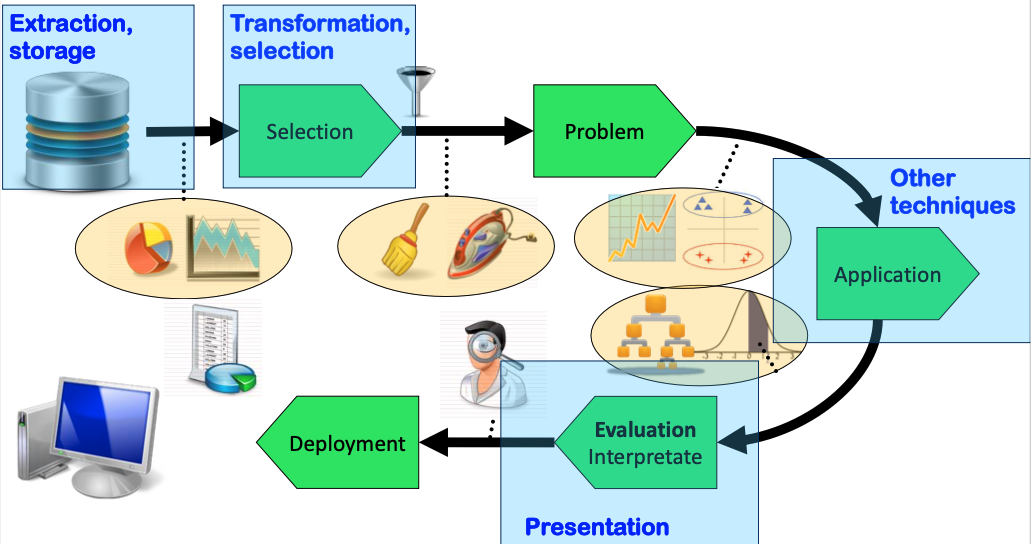
\includegraphics[width=0.7\textwidth]{fotos/4.png}
\caption{Contornos de las funciones de error y ligadura para la regresión Lasso (izquierda) y Ridge (derecha). Las áreas de color azul son las regiones de ligadura $|\beta_1| + |\beta_2| \leq s$ y $\beta_1^2 + \beta_2^2 \leq s$, mientras que las elipses rojas son los contornos del RSS.}
\label{fig:reg}
\end{figure}

\subsubsection{Mejora de Ridge sobre mínimos cuadrados}

La ventaja de la regresión Ridge sobre los mínimos cuadrados se basa en el compromiso entre sesgo y varianza. A medida que $\lambda$ aumenta, la flexibilidad del ajuste de la regresión Ridge disminuye, lo que lleva a una disminución de la varianza pero a un aumento del sesgo. Esto se ilustra en el panel izquierdo de la figura \ref{fig:5}. La curva verde en el panel izquierdo de la Figura 6.5 muestra la varianza de las predicciones de la regresión Ridge como una función de $\lambda$. En las estimaciones de los coeficientes de mínimos cuadrados, que corresponden a la regresión Ridge con $\lambda = 0$, la varianza es alta pero no hay sesgo. Sin embargo, a medida que $\lambda$ aumenta, la contracción de las estimaciones de los coeficientes Ridge conduce a una reducción sustancial de la varianza de las predicciones, a costa de un leve aumento en el sesgo. Recuerda que el error cuadrático medio de prueba (MSE), graficado en púrpura, es una función de la varianza más el sesgo al cuadrado. Para valores de $\lambda$ de hasta aproximadamente 10, la varianza disminuye rápidamente, con un aumento muy leve en el sesgo, graficado en negro. En consecuencia, el error cuadrático medio (MSE) disminuye considerablemente a medida que $\lambda$ aumenta de 0 a 10. Más allá de este punto, la disminución en la varianza debido al aumento de $\lambda$ se ralentiza, y la contracción en los coeficientes causa que se subestimen significativamente, resultando en un gran aumento en el sesgo. El MSE mínimo se alcanza aproximadamente en $\lambda = 30$. Curiosamente, debido a su alta varianza, el MSE asociado con el ajuste de mínimos cuadrados, cuando $\lambda = 0$, es casi tan alto como el del modelo nulo, en el cual todas las estimaciones de los coeficientes son cero, cuando $\lambda \to \infty$. Sin embargo, para un valor intermedio de $\lambda$, el MSE es considerablemente menor.


\begin{figure}[h]
\centering
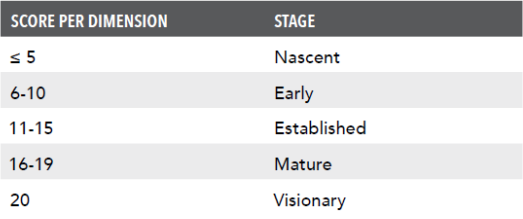
\includegraphics[width=0.8\textwidth]{fotos/5.png}
\caption{\textit{Bias} al cuadrado (negro), varianza (verde) y MSE de \textit{test} (morado) para predicciones de regresión Ridge en un conjunto de datos simulado, como función de $\lambda$ y $||\hat{\beta}_\lambda^R||_2/ ||\hat{\beta}||_2$. La linea discontinua horizontal indica el mínimo MSE posible. Las cruces moradas indican los modelos de regresión Risge para los cuales el MSE es el menor.}
\label{fig:5}
\end{figure}

El panel derecho de la figura \ref{fig:5} muestra las mismas curvas que el panel izquierdo, esta vez graficadas contra la norma $\ell_2$ de las estimaciones de los coeficientes de la regresión Ridge dividida por la norma $\ell_2$ de las estimaciones de mínimos cuadrados. Ahora, a medida que se va de izquierda a derecha, los ajustes se vuelven más flexibles, por lo que el sesgo disminuye y la varianza aumenta. \\

En general, en situaciones donde la relación entre la respuesta y los predictores es casi lineal, las estimaciones por mínimos cuadrados tendrán un sesgo bajo pero pueden tener una alta varianza. Esto significa que un pequeño cambio en los datos de entrenamiento puede causar un gran cambio en las estimaciones de los coeficientes por mínimos cuadrados. En particular, cuando el número de variables $p$ es casi tan grande como el número de observaciones $n$, como en el ejemplo de la figura \ref{fig:5}, las estimaciones por mínimos cuadrados serán extremadamente variables. Y si $p > n$, entonces las estimaciones por mínimos cuadrados ni siquiera tienen una solución única, mientras que la regresión Ridge aún puede funcionar bien al intercambiar un pequeño aumento en el sesgo por una gran disminución en la varianza. Por lo tanto, la regresión Ridge funciona mejor en situaciones donde las estimaciones por mínimos cuadrados tienen alta varianza. \\

Regresión Ridge también tiene una ventaja computacional sobre la elección del mejor subconjunto, que requiere buscar sobre $2^p$ modelos. Para un valor dado de $\lambda$, la regresión Ridge solo ajusta un único modelo. Incluso para valores moderados de $p$, dicha búsqueda puede ser computacionalmente inviable. En contraste, para cualquier valor fijo de $\lambda$, la regresión Ridge solo ajusta un único modelo, y el procedimiento de ajuste del modelo puede realizarse bastante rápido. De hecho, se puede demostrar que los cálculos necesarios para resolver (\ref{eq:6.5}), simultáneamente para todos los valores de $\lambda$, son casi idénticos a los de ajustar un modelo usando mínimos cuadrados. 

\subsection{Regresión Lasso}

La regresión de Ridge tiene una desventaja obvia. A diferencia de la selección del mejor subconjunto, la selección hacia adelante y la selección hacia atrás, que generalmente seleccionan modelos que involucran solo un subconjunto de las variables, la regresión Ridge incluirá todos los $p$ predictores en el modelo final. La penalización $\lambda \sum \beta_j^2$ en (\ref{eq:6.5}) reducirá todos los coeficientes hacia cero, pero no establecerá ninguno de ellos exactamente en cero (a menos que $\lambda = \infty$). Esto puede no ser un problema para la precisión de la predicción, pero puede crear un desafío en la interpretación del modelo en contextos donde el número de variables $p$ es bastante grande. Sin embargo, se puede querer un modelo que incluya solo los predictores más relevantes. \\

Lasso es una alternativa relativamente reciente a la regresión de Ridge que supera esta desventaja. Los coeficientes de Lasso, $\hat{\beta}^{L}_{\lambda}$, minimizan la cantidad
\begin{equation}
\sum_{i = 1}^n \left(y_i - \beta_0 - \sum_{j=1}^p \beta_j x_{ij}\right)^2 + \lambda \sum_{j=1}^p |\beta_j| = \text{RSS} + \lambda \sum_{j=1}^p |\beta_j| 
\label{eq:6.7}
\end{equation}

\noindent Esto puede escribirse como 
\begin{align}
\underset{\boldsymbol{\beta}}{\text{minimize}} \quad &\sum_{i=1}^{n}\left(y_i - \beta_0 - \sum_{j=1}^{p}\beta_j x_{ij}\right)^2 \\
\text{sujeto a} \quad &\sum_{j=1}^{p}|\beta_j| \leq s \label{eq:6.9}
\end{align}

Comparando (\ref{eq:6.7}) con (\ref{eq:6.5}), se ve que Lasso y Ridge tienen formulaciones similares. La única diferencia es la condición de ligadura. En términos estadísticos, Lasso usa una penalización $\ell_1$ en lugar de la $\ell_2$. La norma $\ell_1$ de un vector de coeficientes $\beta$ viene dada por $||\beta||_1 = \sum |\beta_j|$. \\

Al igual que en la regresión Ridge, Lasso reduce las estimaciones de los coeficientes hacia cero. Sin embargo, en el caso de Lasso, la penalización $\ell_1$ tiene el efecto de forzar que algunas de las estimaciones de los coeficientes sean exactamente cero cuando el parámetro de ajuste $\lambda$ es suficientemente grande. Por lo tanto, al igual que la selección del mejor subconjunto, Lasso realiza una selección de variables. Como resultado, los modelos generados por Lasso son generalmente mucho más fáciles de interpretar que los producidos por la regresión Ridge. Se dice que Lasso produce modelos escasos (\textit{sparse}) decir, modelos que involucran solo un subconjunto de las variables. Al igual que en la regresión Ridge, seleccionar un buen valor de $\lambda$ para Lasso es crucial.

\begin{figure}[h]
\centering
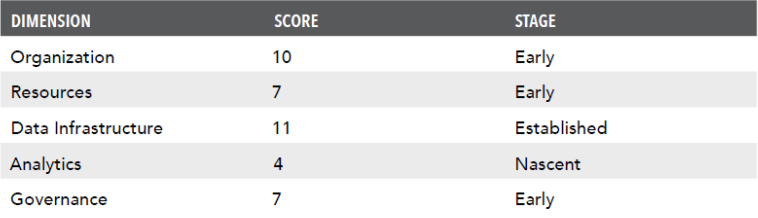
\includegraphics[width=0.8\textwidth]{fotos/6.png}
\caption{Ejemplo de coeficientes Lasso en un \textit{dataset} como función de $\lambda$ y $||\hat{\beta}_\lambda^L||_1 / ||\hat{\beta}||_1$. Cuando $\lambda = 0$, Lasso proporciona el ajuste de mínimos cuadrados, y cuando $\lambda$ se vuelve suficientemente grande, Lasso da el modelo nulo en el que todas las estimaciones de los coeficientes son iguales a cero. Sin embargo, entre estos dos extremos, los modelos de regresión Ridge y Lasso son bastante diferentes entre sí. Moviéndose de izquierda a derecha en el panel derecho, se observa que al principio Lasso resulta en un modelo que contiene solo el predictor \textit{rating}. Luego, \textit{student} y \textit{limit} entran en el modelo casi simultáneamente, seguidos poco después por \textit{income}. Eventualmente, las variables restantes entran en el modelo. Por lo tanto, dependiendo del valor de $\lambda$, Lasso puede producir un modelo que involucre cualquier número de variables. En contraste, la regresión Ridge siempre incluirá todas las variables en el modelo, aunque la magnitud de las estimaciones de los coeficientes dependerá de $\lambda$.}
\label{fig:6.6}
\end{figure}

\subsubsection{Propiedad de selección de variables en Lasso}

¿Por qué Lasso, a diferencia de la regresión Ridge, resulta en estimaciones de coeficientes que son exactamente iguales a cero? Las formulaciones (\ref{eq:6.8}) y (\ref{eq:6.9}) pueden usarse para arrojar luz sobre el asunto. La figura \ref{fig:reg} ilustra la situación. La solución de mínimos cuadrados está marcada como $\hat{\beta}$, mientras que el diamante y círculo azul representan las restricciones de Lasso y Ridge en (\ref{eq:6.8}) y (\ref{eq:6.9}), respectivamente. Si $s$ es suficientemente grande, entonces las regiones de restricción contendrán $\hat{\beta}$, y por lo tanto, las estimaciones de regresión Ridge y Lasso serán las mismas que las estimaciones de mínimos cuadrados (un valor tan grande de $s$ corresponde a $\lambda = 0$ en (\ref{eq:6.5}) y (\ref{eq:6.7})). Sin embargo, en la figura \ref{fig:reg} las estimaciones de mínimos cuadrados se encuentran fuera del diamante y del círculo, y por lo tanto, las estimaciones de mínimos cuadrados no son las mismas que las estimaciones de Lasso y regresión Ridge. \\

Las elipses que están centradas alrededor de $\hat{\beta}$ representan regiones de RSS constante. En otras palabras, todos los puntos en una elipse dada comparten un valor común del RSS. A medida que las elipses se expanden alejándose de las estimaciones de los coeficientes de mínimos cuadrados, el RSS aumenta. Las ecuaciones (\ref{eq:6.8}) y (\ref{eq:6.9}) indican que las estimaciones de los coeficientes de Lasso y regresión Ridge están dadas por el primer punto en el que una elipse contacta la región de restricción. Dado que la regresión Ridge tiene una restricción circular sin puntos agudos, esta intersección generalmente no ocurrirá en un eje, y por lo tanto, las estimaciones de los coeficientes de regresión Ridge serán exclusivamente diferentes de cero. Sin embargo, la restricción de Lasso tiene esquinas en cada uno de los ejes, y por lo tanto, la elipse a menudo intersectará la región de restricción en un eje. Cuando esto ocurre, uno de los coeficientes será igual a cero. En dimensiones más altas, muchas de las estimaciones de los coeficientes pueden ser iguales a cero simultáneamente. En la figura \ref{fig:reg}, la intersección ocurre en $\beta_1 = 0$, y por lo tanto, el modelo resultante solo incluirá $\beta_2$. \\

En la figura \ref{fig:reg}, se considera el caso simple de $p = 2$. Cuando $p = 3$, la región de restricción para la regresión Ridge se convierte en una esfera, y la región de restricción para el lasso se convierte en un poliedro. Cuando $p > 3$, uno de los coeficientes será igual a cero. En dimensiones más altas, muchas de las estimaciones de los coeficientes pueden ser iguales a cero simultáneamente. En la figura \ref{fig:reg}, la intersección ocurre en $\beta_1 = 0$, y por lo tanto, el modelo resultante solo incluirá $\beta_2$. \\

En la figura \ref{fig:reg}, se considera el caso simple de $p = 2$. Cuando $p = 3$, la restricción para la regresión Ridge se convierte en una hiperesfera, y la región de restricción para Lasso se convierte en un politopo. Sin embargo, las ideas clave representadas en la figura \ref{fig:reg} siguen siendo válidas. En particular, Lasso conduce a la selección de características cuando $p > 2$ debido a las esquinas agudas del poliedro o politopo.

\subsubsection{Comparación entre regresión Lasso y Ridge}

\begin{figure}[h]
\centering

\includegraphics[width=0.8\textwidth]{fotos/7.png}
\caption{Izquierda: Gráficas del sesgo cuadrado (negro), varianza (verde) y MSE de prueba (morado) para Lasso en un conjunto de datos simulado. Los datos simulados son similares a los de la figura \ref{fig:6.8}, excepto que ahora solo dos predictores se relacionan con la respuesta. Derecha: Comparación del sesgo cuadrado, varianza y MSE de prueba entre Lasso (sólido) y Ridge (discontinuo). Ambos se grafican contra su $R^2$ en los datos de entrenamiento, como una forma común de indexación. Las cruces en ambas gráficas indican el modelo Lasso para el cual el MSE es el más pequeño.}
\label{fig:6.8}
\end{figure}

Es claro que Lasso tiene una ventaja importante sobre la regresión Ridge, ya que produce modelos más simples y más interpretables que involucran solo un subconjunto de los predictores. Sin embargo, ¿qué método conduce a una mejor precisión de predicción? La figura \ref{fig:6.8} muestra la varianza, el sesgo cuadrado y el MSE de prueba del lasso aplicado a los mismos datos simulados que en la figura \ref{fig:5}. Claramente, Lasso conduce a un comportamiento cualitativamente similar al de la regresión Ridge, en el sentido de que a medida que $\lambda$ aumenta, la varianza disminuye y el sesgo aumenta. En el panel derecho de la figura \ref{fig:6.8}, las líneas punteadas representan los ajustes de la regresión Ridge. Aquí se grafican ambos contra su $R^2$ en los datos de entrenamiento. Esta es otra forma útil de indexar modelos, y puede usarse para comparar modelos con diferentes tipos de regularización, como es el caso aquí. En este ejemplo, Lasso y la regresión Ridge resultan en sesgos casi idénticos. Sin embargo, la varianza de la regresión Ridge es ligeramente menor que la varianza del lasso. En consecuencia, el MSE mínimo de la regresión Ridge es ligeramente menor que el de Lasso. \\

Sin embargo, los datos en la figura \ref{fig:6.8} fueron generados de tal manera que todos los 45 predictores estaban relacionados con la respuesta, es decir, ninguno de los coeficientes verdaderos $\beta_1, \ldots, \beta_{45}$ era igual a cero. Lasso asume implícitamente que varios de los coeficientes son realmente iguales a cero. En consecuencia, no es sorprendente que la regresión Ridge supere a Lasso en términos de error de predicción en este contexto. La Figura \ref{fig:6.9} ilustra una situación similar, excepto que ahora la respuesta es una función de solo 2 de los 45 predictores. Ahora, Lasso tiende a mejorar la actuación de la regresión Ridge en términos de sesgo, varianza y MSE. 

\begin{figure}[h]
\centering
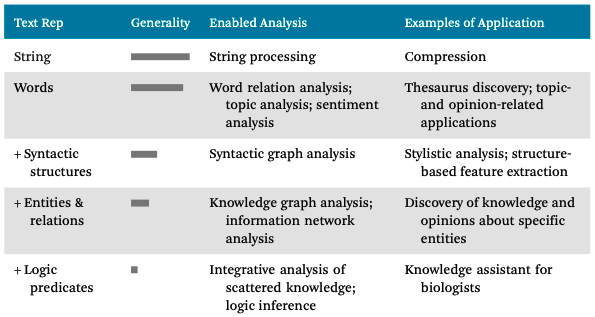
\includegraphics[width=0.8\textwidth]{fotos/8.png}
\caption{Izquierda: Gráficas del sesgo cuadrado (negro), varianza (verde) y MSE de prueba (morado) para Lasso en un conjunto de datos simulado. Derecha: Comparación del sesgo cuadrado, varianza y MSE de prueba entre Lasso (sólido) y Ridge (discontinuo). Ambos se grafican contra su $R^2$ en los datos de entrenamiento, como una forma común de indexación. Las cruces en ambas gráficas indican el modelo Lasso para el cual el MSE es el más pequeño.}
\label{fig:6.9}
\end{figure}

Estos dos ejemplos ilustran que ni la regresión Ridge ni Lasso dominarán al otro. En general, uno podría esperar que Lasso funcione mejor en un contexto donde un número relativamente pequeño de predictores tenga coeficientes sustanciales, y los predictores restantes tengan coeficientes muy pequeños o iguales a cero. La regresión Ridge funcionará mejor cuando la respuesta sea una función de muchos predictores, todos con coeficientes de tamaño aproximadamente igual. Sin embargo, el número de predictores que está relacionado con la respuesta nunca se conoce a priori para conjuntos de datos reales. Una técnica como la validación cruzada puede usarse para determinar qué enfoque es mejor en un conjunto de datos particular. \\ 

Al igual que en la regresión Ridge, cuando las estimaciones de mínimos cuadrados tienen una varianza excesivamente alta, la solución de Lasso puede producir una reducción en la varianza a expensas de un pequeño aumento en el sesgo y, en consecuencia, puede generar predicciones más precisas. A diferencia de la regresión Ridge, Lasso realiza una selección de variables y, por lo tanto, resulta en modelos que son más fáciles de interpretar.

\subsection{Selección del parámetro de ajuste}

Al igual que los enfoques de selección de subconjuntos considerados en la sección \ref{sec:4.1} requieren un método para determinar cuál de los modelos en consideración es el mejor, implementar la regresión Ridge y Lasso requiere un método para seleccionar un valor para el parámetro de ajuste $\lambda$ en (\ref{eq:6.5}) y (\ref{eq:6.7}), o, de manera equivalente, el valor de la restricción $s$ en (\ref{eq:6.8}) y (\ref{eq:6.9}). La validación cruzada proporciona una forma sencilla de abordar este problema. Se elige una cuadrícula de valores de $\lambda$ y se calcula el error de validación cruzada para cada valor de $\lambda$. Luego se selecciona el valor del parámetro de ajuste para el cual el error de validación cruzada es el más pequeño. Finalmente, el modelo se vuelve a ajustar utilizando todas las observaciones disponibles y el valor seleccionado del parámetro de ajuste. 

\textcolor{red}{FALTA PROBLEMAs en alta dimension !!!!}

\section{Reducción de dimensión}

El análisis de componentes principales (PCA) es un enfoque popular para derivar un conjunto de características de baja dimensión a partir de un gran conjunto de variables. Aquí se describe su uso como una técnica de reducción de dimensión para la regresión.

\subsection{Análisis de componentes principales}

\subsubsection{Una única muestra}

Para un vector aleatorio $X = (X_1, \dots, X_p)^T$, el vector de medias es $\boldsymbol{\mu} = (\mu_1, \dots, \mu_p)^T$, y la matriz de covarianza de la población $\Sigma$ viene dada por 
\begin{equation}
\Sigma = \begin{pmatrix}
\text{Var}(X_1) & \text{Cov}(X_1, X_2) & \cdots & \text{Cov}(X_1, X_p) \\
\text{Cov}(X_2, X_1) & \text{Var}(X_2) & \cdots & \text{Cov}(X_2, X_p) \\
\vdots & \vdots & \ddots & \vdots \\
\text{Cov}(X_p, X_1) & \text{Cov}(X_p, X_2) & \cdots & \text{Var}(X_p)
\end{pmatrix}
\end{equation}

Sean $\lambda_1 \geq \lambda_2  \geq \dots \geq \lambda_p \geq 0$ los autovalores de $\Sigma$, y $\mathbf{e}_1, \dots, \mathbf{e}_p$ los correspondientes vectores propios (debidamente normalizados). La varianza de la componente principal k-ésima será igual a $\lambda_k$, mientras que los elemetnos de $\mathbf{e}_k$ serán los coeficientes de la componente principal k-ésima. La primera componente principal será la que mayor varianza tenga, y su autovalor será el mayor. \\

\noindent La proporción de varianza explicada por la componente principal k-ésima es 
\begin{equation}
\frac{\lambda_k}{\sum_{j=1}^p \lambda_j}
\end{equation}

\noindent Por tanto, la proporción de varianza explicada por las $M$ primeras componentes principales es
\begin{equation}
\frac{\sum_{j=1}^M \lambda_j}{\sum_{j=1}^p \lambda_j}
\end{equation}

\noindent La matriz de correlación será 
\begin{equation}
\rho = \begin{pmatrix}  
1 & \rho_{12} & \cdots & \rho_{1p} \\
\rho_{21} & 1 & \cdots & \rho_{2p} \\
\vdots & \vdots & \ddots & \vdots \\
\rho_{p1} & \rho_{p2} & \cdots & 1
\end{pmatrix}, \quad \rho_{ij} = \frac{\sigma_{ij}}{\sigma_i \sigma_j} = \frac{\text{Cov}(X_i, X_j)}{\sqrt{\text{Var}(X_i) \text{Var}(X_j)}}
\end{equation}

\noindent donde $\rho_{ij}$ es la correlación entre las variables $X_i$ y $X_j$


\subsubsection{n muestras}

Sea un conjunto de $n$ observaciones y $p$ características $X_1, X_2, \ldots, X_p$, 
\begin{equation}
X = \begin{pmatrix}
x_{11} & x_{12} & \cdots & x_{1p} \\
x_{21} & x_{22} & \cdots & x_{2p} \\
\vdots & \vdots & \ddots & \vdots \\
x_{n1} & x_{n2} & \cdots & x_{np}
\end{pmatrix}
\label{eq:pr1}
\end{equation}

Las componentes de este conjunto suelen ser dependientes y contienen información redundante. Por tanto, podría resultar útil tomar combinaciones lineales de las variables originales, manteniendo la mayor cantidad de información posible. Cada una de las $n$ observaciones yace en un espacio de $p$ dimensiones, y el objetivo del PCA es proyectar estos datos en un espacio de menor dimensión que contenga la mayor cantidad de variabilidad en los datos. \\

Si ahora se toma un conjunto de $n$ observaciones y $p$ características (\ref{eq:pr1}), se puede estimar $\boldsymbol{\mu}$ como $\bar{x} = (\bar{x}_1, \dots, \bar{x}_p)^T$, y la matriz de covarianza como 
\begin{equation}
S = \begin{pmatrix}
s_1^2 & s_{12} & \cdots & s_{1d} \\
s_{21} & s_2^2 & \cdots & s_{2d} \\
\vdots & \vdots & \ddots & \vdots \\
s_{d1} & s_{d2} & \cdots & s_d^2
\end{pmatrix}
\end{equation}

El análisis de componentes principales se centra en explicar la estructura de varianza-covarianza de $X = (X_1, \dots, X_p)^T$ a partir de un conjunto menor de variables no correlacionadas (las componentes principales). Las componentes principales $Z$ son combinaciones lineales no correlacionadas de las características $X_1, \dots, X_p$ y cuya varianza es lo más grande posible. Matemáticamente, las componentes principales son 
\begin{equation}
Z_m = \phi_{m1}X_1 + \phi_{m2}X_2 + \dots + \phi_{mp}X_p = \boldsymbol{\phi}_m^T X
\end{equation}

maximizando $\text{Var}(Z_1) = \boldsymbol{\phi}_m^T S \boldsymbol{\phi}_m$ sujeto a $||\boldsymbol{\phi}_m|| = \sum_{j=1}^p \phi_{jm}^2 = 1$ y $\text{Cov} (Z_k, Z_m) = \boldsymbol{\phi}_k^T S \boldsymbol{\phi}_m = 0$ para $m < k$. \\

\noindent En este caso, se puede estimar la matriz de covarianza con la matriz de correlación muestral, 
\begin{equation}
R = \begin{pmatrix}
1 & r_{12} & \cdots & r_{1p} \\
r_{21} & 1 & \cdots & r_{2p} \\
\vdots & \vdots & \ddots & \vdots \\
r_{p1} & r_{p2} & \cdots & 1
\end{pmatrix}, \quad r_{ij} = \frac{s_{ij}}{s_i s_j}
\end{equation}

\subsection{Regresión de componentes principales}

El análisis de componentes principales puede usarse como método de reducción de dimensión en problemas de regresión. Sea una respuesta cuantitativa $Y$ y un conjunto de predictores $\mathbf{X} = (X_1, \dots, X_p)^T$. La regresión de componentes principales se basa en construir las primeras $M$ componentes principales $Z_1, \dots, Z_M$ y luego usarlas como predictores en un modelo de regresión lineal ajustado con mínimos cuadrados, 
\begin{equation}
Y = \beta + \sum_{i=1}^M \beta_i Z_i + \epsilon
\end{equation}

Esta técnica asume que las direcciones en las que $X_1, \dots, X_p$ muestran mayor variabilidad son las direcciones asociadas con $Y$, las más importantes a la hora de predecirla. La estimación de $k \ll p$ puede resolver problemas de \textit{overfitting}.

\subsection{Consideraciones en PCA}

\subsubsection{Escalado de variables}

Antes de realizar el PCA, las variables deben centrarse para tener una media de cero (la media por columnas de $\mathbf{X}$ debe ser 0). Además, los resultados obtenidos al realizar el PCA también dependerán de si las variables se han escalado individualmente (cada una multiplicada por una constante diferente). Esto contrasta con algunas otras técnicas de aprendizaje supervisado y no supervisado, como la regresión lineal, en las que escalar las variables no tiene efecto. \\

Además, resulta poco deseable que las componentes principales obtenidas dependan de una elección arbitraria de escala, por lo que se suele escalar cada variable para tener desviación estándar unitaria antes de realizar el PCA. Sin embargo, si las variables están medidas en las mismas unidades, este escalado no es necesario.

\begin{figure}[h]
\centering
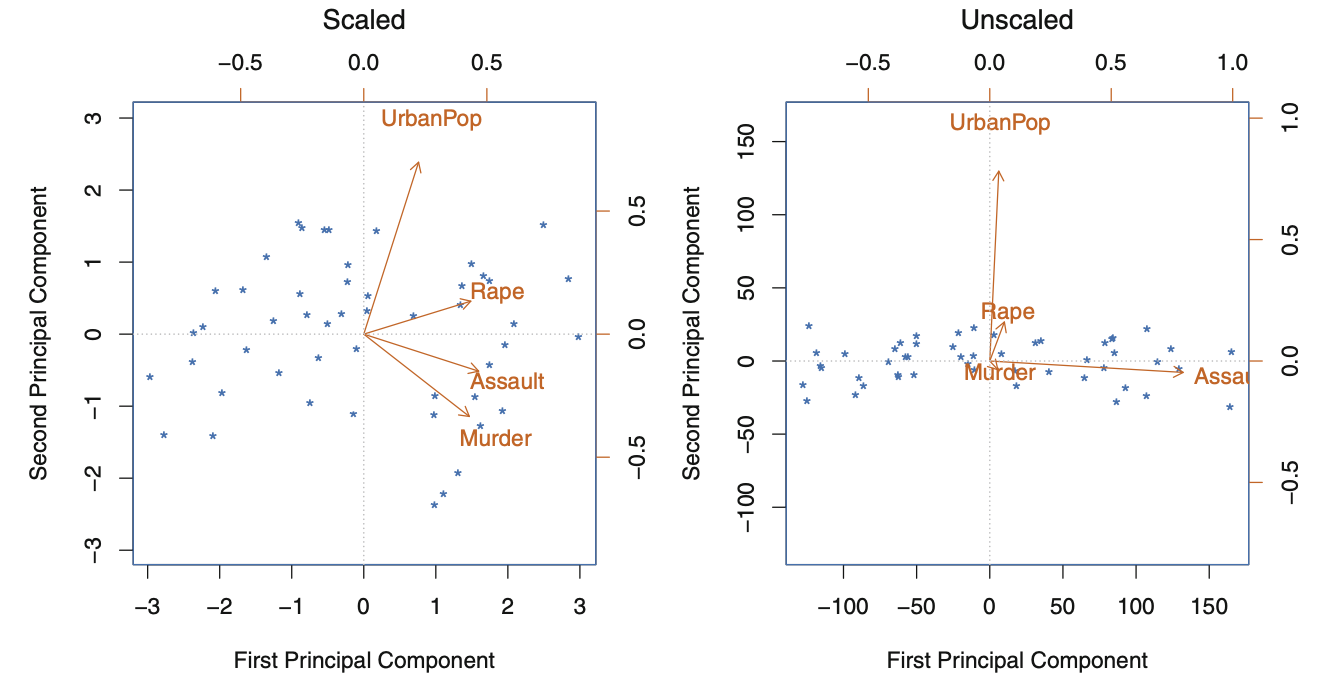
\includegraphics[width=\textwidth]{fotos/19.png}
\caption{Dos biplots de componentes principales para los datos de \textit{USArrests}. Variables escaladas para tener desviaciones estándar unitarias. Derecha: componentes principales usando datos no escalados. \textit{Assault} tiene, con diferencia, la mayor carga en el primer componente principal porque tiene la mayor varianza entre las cuatro variables. En general, se recomienda escalar las variables para que tengan una desviación estándar de uno.}
\label{fig:10.3}
\end{figure}

\subsubsection{Unicidad de las componentes principales}

Cada vector de cargas de los componentes principales es único, salvo un cambio de signo. Los signos pueden diferir porque cada vector de cargas de los componentes principales especifica una dirección en el espacio p-dimensional: cambiar el signo no tiene efecto ya que la dirección no cambia.